\chapter{Model validation}
The validation of the model was done by measuring the output equivalent resistance of a SCC and comparing to the model results, either using transient circuit simulations and experimental circuits.

Because the proposed method has the goal to model losses produced by the charge transfer between capacitors and conductance through resistive elements (switches and parasitics), simulations with a behavioral simulator only take into account these two sources of losses, enabling a fair comparison to validate the proposed model.  Nevertheless, an experimental converter was specifically build with the only propose to validate measure and validate the model. The converter was designed to mitigate any other source of loss not included in the model, such as switching losses. These other loss mechanisms, such as switching losses, can be added to the model as described in ~\cite{Seeman:EECS-2009-78}; however, they are out of the scope of the model presented in the previous chapter.

This chapter is divided in three sections. The first section presenters the setup used to measure the $r_{scc}$ of a converter, which is the same for an experimental or a simulation circuit. The second section is devoted to the validation using transient circuit simulations, providing a through analysis of the results thanks to the flexibility of using circuit simulations. The last chapter introduces the experimental prototype and the obtained measurements.


\section{Measuring $r_{scc}$ from a SCC}
In both cases, it has been used the same configuration to measure the equivalent output resistance, as depicted in Figure~\ref{fig:rscc_exp_setup}. In the experimental arrangement, two Keithley\textsuperscript{\textregistered} \emph{SourceMeter 2440} were used to measure currents, and two Keithley\textsuperscript{\textregistered} \emph{Meters 2000} were used to measure the voltages.

\begin{figure}[!h]
\centering
\ctikzset { bipoles/length=1cm}
\begin{circuitikz}[american,scale=0.65]
\draw
    (2.5,0) to[short]
    (-1.5,0) to[V = $v_{src}$]
    (-1.5,3) to[ammeter,l=$i_{in}$]  (1,3) -- (2.5,3)
    (1,3) to[voltmeter,l_=$v_{in}$] (1,0);


\draw [thick]
    (2.5,-0.5) --
    (2.5,3.5)  --
    (5.5,3.5)  --
    (5.5,-0.5) --
    (2.5,-0.5);

\draw (4,2) node[anchor=north,align=center]{SCC \\ U.T.} ;

\draw
    (5.5,3) --
    (7,3) to[ammeter,l=$i_{out}$]
    (9.5,3) to[switch,l=$s_1$]  (10,3) -- (10.5,3) to[I,l = $i_{load}$]
    (10.5,0) -- (5.5,0)
    (7,3) to[voltmeter,l^=$v_{out}$] (7,0);
\end{circuitikz}
\caption{Experimental arrangement used to test and measure the characteristics of an SCC. }
\label{fig:rscc_exp_setup}
\end{figure}

$r_{scc}$ is computed in two steps, operating the converter with the same values of $f_{sw}$ and $D$:
\begin{enumerate}
  \item Operating with no load ($s_1$ open), the \emph{target voltage} ($v_{trg}$) and the conversion ration $m$ are determined,
      \begin{align}
        v_{trg} & = v_{out},\label{eq:vtrg}\\
        m & = \frac{v_{out}}{v_{in}}.
        \label{eq:vtrg_m}
      \end{align}

  \item Loading the converter with constant current ($s_1$ closed),  $r_{scc}$ is computed using~\eqref{eq:vtrg},
      \begin{equation}
        r_{scc} = \frac{v_{trg} - v_{out}}{i_{out}}.
        \label{eq:rscc_m}
      \end{equation}
\end{enumerate}


\begin{figure}[t]
\ctikzset { bipoles/length=1cm}
\centering
\begin{subfigure}[t]{0.45\textwidth}
    \centering
    \begin{circuitikz}[american,scale=0.6]
    \draw
            %Input Supply
            %(0,0)  to[V=$v_{src}$]
            %Draw Switches
            %(0,10)  --
            (5,10.3) node[anchor=south] {$v_{src}$}
            (5,10) node[rground, yscale=-1] {}
            to[switch=$s_1$] %S1
            (5,8)   to[switch=$s_2$] %S2
            (5,6)   to[switch=$s_3$] %S3
            (5,4) --
            %left branch
            (3,4)   to[switch=$s_7$]
            (3,2)   to[switch=$s_6$]
            (3,0);

    \draw   %right branch
            (5,4) --
            (7,4)   to[switch,l_=$s_4$]
            (7,2)   to[switch,l_=$s_5$]
            (7,0) -- (3,0);


    \draw %Capacitor C1
           (3,2) -- (2,2) -- (2,4)
            to[pC,l_=$c_1$] (2,8) --
           (5,8);

    \draw %Capacitor C2
           (7,2) --
           (8.25,2) -- (8.25,3.5)  to[pC,l^=$c_2$] (8.25,6) --
           (5,6);

    \draw %Capacitor C3
           (5,0) node[sground] {} to[pC,l_=$c_3$] (5,4);

     %\draw (7,4) to[short,-o] (10,4) node[anchor=west] {};

     %\draw (9,6) to[open,v^=$v_{1}$] (9,0);
     %\draw (8.25,6) to[short,-o] (9,6) node[anchor=west] {$v_{out}$} ;
     \draw (8.25,6) -- (9.5,6) to[I,l^=$i_{out}$] (9.5,0) |- (5,0);
     \end{circuitikz}
\caption{}
\label{fig:3_1_hscc_exp_a}
\end{subfigure}
\hfill
\hfill
\begin{subfigure}[t]{0.45\textwidth}
    \centering
    \begin{circuitikz}[american ,scale=0.6]
    \draw
            %Input Supply
            %(0,0)  to[V=$v_{src}$]
            %Draw Switches
            %(0,10)  --
            (5,10.3) node[anchor=south] {$v_{src}$}
            (5,10) node[rground, yscale=-1] {}
            to[switch=$s_1$] %S1
            (5,8)   to[switch=$s_2$] %S2
            (5,6)   to[switch=$s_3$] %S3
            (5,4) --
            %left branch
            (3,4)   to[switch=$s_7$]
            (3,2)   to[switch=$s_6$]
            (3,0);

    \draw   %right branch
            (5,4) --
            (7,4)   to[switch,l_=$s_4$]
            (7,2)   to[switch,l_=$s_5$]
            (7,0) -- (3,0);


    \draw %Capacitor C1
           (3,2) -- (2,2) -- (2,4)
            to[pC,l_=$c_1$] (2,8) --
           (5,8);

    \draw %Capacitor C2
           (7,2) --
           (8.25,2) -- (8.25,3.5)  to[pC,l^=$c_2$] (8.25,6) --
           (5,6);

    \draw %Capacitor C3
           (5,0) node[sground] {} to[pC,l_=$c_3$] (5,4);

     %\draw (7,4) to[short,-o] (10,4) node[anchor=west] {};

     %\draw (9,6) to[open,v^=$v_{1}$] (9,0);
     \draw (5,4)  --([hs]8.25,4 |- 5,4) arc(180:0:\radius) to[short] (9.5,4) to[I,l^=$i_{out}$] (9.5,0) |- (5,0);
     \end{circuitikz}
\caption{}
\label{fig:3_1_hscc_exp_b}
\end{subfigure}
\caption{Test circuits 3:1 Dickson used for model validation: \emph{left}- output taken from a \emph{pwm}-node; \emph{right}- output taken from a \emph{dc}-node.}
\label{fig:3_1_hscc_exp}
\end{figure}

The model was validated using a 3:1 Dickson converter for the two different scenarios presented in Figure~\ref{fig:3_1_hscc_exp}. In the first scenario, the load is connected to the second \emph{pwm}-node, Figure~\ref{fig:3_1_hscc_exp_a}. In the other scenario, the converter is loaded at the \emph{dc}-node, Figure~\ref{fig:3_1_hscc_exp_b}. In both cases the output impedance values are compared with results obtained from transient PLECS\footnote{\label{fn:PLECS}Behavioral circuit simulator} simulations. Furthermore results from the second scenario are compared with results from previous modeling works.  A detailed example in how to solve the circuits and the charge flow vectors $\mathbf{a}, \mathbf{b} $ and $\mathbf{ar}$ are presented in the Appendix~\ref{apx:31_dick_charge_flows}.


%
%Only transient circuit simulations in PLECS have been used for the initial assessment and validation of the modeling work. Actually, the presented modeling has the goal to model losses produced by the charge transfer between capacitors and by conductance through resistive elements , which are the many source of losses in a SCC that mainly determine the values for capacitors and switches. By using a transient circuit simulator, we can simulate a SCC which can produce only these two source of losses, thus only reproducing studied phenomena of the models. Other source of losses such as switching losses, bottom-plate capacitors losses or driving losses, are beyond this works scope since they have been already studied and
%reported and they can be easily included in the model.

The values for capacitors $c_1$,$c_2$ and $c_3$ are 100nF and all switches have the same \emph{on}-channel resistance of $100m\Omega$. The circuits were supplied at $10V$ and the load current $i_{out}$ was adjusted in each simulation depending on the operation point of the converter, keeping the efficiency to $\eta=95\%$, by using the following expression
\begin{equation}
    i_{out}=m_x~v_{src}\frac{1-\eta}{r_{scc,mdl}},
\label{eq:iout_eff}
\end{equation}
where $m_x$ was the conversion ratio for the given output and $r_{scc,mdl}$ was obtained using the model. Fixing a constant efficiency and high enough, guarantees a similar average output voltage across all the simulations, indeed rearranging~\eqref{eq:eff_vo} yelds
\begin{equation}
    v_{out}=m_x~v_{src}~\eta,
\label{eq:vout_eff}
\end{equation}
where $m_x$ is the conversion ration for the $x$ output.

\subsubsection{ Floating \emph{pwm}-output }
Figures~\ref{fig:exp_rscc_pwm_node_dx} and~\ref{fig:exp_rscc_pwm_node_fsw} present the results of $r_{scc}$ for a sweep of the duty cycle ($D$) and frequency ($f_{sw}$) respectively. In both figures, the results from the model are obtained using the presented methodology in this chapter, however results are for different $r_{scc}$ approximations described in Section~\ref{ch:rscc_apprx}.

Figure~\ref{fig:exp_rscc_pwm_node_dx} presents a sweep in duty cycle for different frequencies, respectively: $100kHz$, $1MHz$, $10MHz$ and $100MHz$. The two extreme cases, top and bottom, present the highest accuracy between the model and the simulation results with less than $2\%$ of error, because the converter operate in the deep regions of the two well-defined operation limits: SSL (Figure~\ref{fig:exp_rscc_pwm_node_100kHz}) and FSL (Figure~\ref{fig:exp_rscc_pwm_node_100MHz}). Outside the deep operation limits (Figures~\ref{fig:exp_rscc_pwm_node_1MHz} and~\ref{fig:exp_rscc_pwm_node_10MHz}), the accuracy is dramatically decreased increasing up to an order of magnitude. The origin for this inaccuracy is due to of the used approximation methods used to compute $r_{scc}$; besides the new proposed approximations, the original formula ($r_{scc} = \sqrt{r_{ssl}^2 + r_{fsl}^2}$) presents to best results. Independently of the model accuracy, it can be seen that predictive trends (in all fourth plots of Figure~\ref{fig:exp_rscc_pwm_node_dx}) are still consistent for variations in duty cycle.

%Looking at the trends with respect to the duty cycle, we can identify that all plots have a tendency to decreases the value of $r_{scc}$ as the duty cycle increases. Actually, higher values of $D$ make switch $s_2$ to conduct for longer periods of time,
Figure~\ref{fig:exp_rscc_pwm_node_fsw} presents $r_{scc}$ foe a sweep of the switching frequency ($f_{sw}$,), showing the well-known characteristic curve. Results are presented  for different duty cycles. Consistent with the previous results, the accuracy is always reduced in the elbow of the curve where the converter operates in between the two limiting regions. At the same time, extreme duty cycles show smaller relative error ($\epsilon_r$). However this smaller values in $\epsilon_r$ are also influenced by the higher values of $r_{scc}$ at these regions.  Looking to the different approximations of $r_{scc}$, as in the previous case, the original formulation still obtains the best accuracy.

\begin{figure}[!h]
\centering
    \begin{subfigure}{\textwidth}
        \parbox[c]{.03\linewidth}{\subcaption{}\label{fig:exp_rscc_pwm_node_100kHz}}
        \hspace{.02\linewidth}
        \parbox[c]{.95\linewidth}{
        \centering
        % This file was created by matlab2tikz.
%
%The latest updates can be retrieved from
%  http://www.mathworks.com/matlabcentral/fileexchange/22022-matlab2tikz-matlab2tikz
%where you can also make suggestions and rate matlab2tikz.
%

\begin{tikzpicture}
\pgfplotsset{
    width=9cm,
    height=2.5cm,
    scale only axis,
    xlabel near ticks,
    ylabel near ticks,
    enlarge y limits={0.2},
    legend style={
                legend columns = 3,
                at={(0.5,1.075)},
                anchor=south,
                draw=none,
                font=\small,
                column sep=2ex,
                legend cell align=left},
}

\begin{axis}[%
    axis x line*=bottom,
    axis y line*=left,
    %xlabel= {duty cycle},
    ylabel= {$r_{scc}~[\Omega]$},
    yticklabel style={text width=2em,align=right},
    ]
    
    \addplot [semithick,mark=square,only marks,white]
      table[y=y1] {./3_modeling/rx_sw_dx_O1.dat};\label{pl_PLECS_hidden}

    \addplot [semithick,mark=square,only marks]
      table[y=y1] {./3_modeling/rx_sw_dx_O1.dat};\label{pl_PLECS}


    \addplot [semithick,smooth,mark=o,mark repeat=10]
      table [y=y1] {./3_modeling/rm1_sw_dx_O1.dat};\label{pl_MDL_JD}

    \addplot [semithick,smooth,mark=+,mark repeat=10]%black!66]
      table [y=y1] {./3_modeling/rm2_sw_dx_O1.dat};\label{pl_Makw}

    \addplot [semithick,smooth,mark=x,mark repeat=10]%black!33]
      table [y=y1] {./3_modeling/rm3_sw_dx_O1.dat};\label{pl_Makw rec}



\end{axis}

\begin{axis}[%
    axis y line*=right,
    axis x line=none,
    ylabel = {$\epsilon_r~[\%]$},
    yticklabel pos=right,
    yticklabel style={text width=2em,align=left},
    ]
    \addlegendimage{/pgfplots/refstyle=pl_PLECS}\addlegendentry{PLECS}
    \addlegendimage{/pgfplots/refstyle=pl_MDL_JD}\addlegendentry{This Work}

    \addplot [semithick,mark=o,only marks,black!60]
      table [y=y1] {./3_modeling/err1_sw_dx_O1.dat};
    \addlegendentry{ $\epsilon_r$ (Rel. Error)}


    \addlegendimage{/pgfplots/refstyle=pl_PLECS_hidden}\addlegendentry{\color{white}PLECS}
    \addlegendimage{/pgfplots/refstyle=pl_Makw}\addlegendentry{Makowski}
    \addplot [semithick,mark=+,only marks,black!60]
      table [y=y1] {./3_modeling/err2_sw_dx_O1.dat};
    \addlegendentry{$\epsilon_r$ \color{white}(Rel. Error) }

    \addlegendimage{/pgfplots/refstyle=pl_PLECS_hidden}\addlegendentry{\color{white}PLECS}
    \addlegendimage{/pgfplots/refstyle=pl_Makw rec}\addlegendentry{Mak. rect.}
    \addplot [semithick,mark=x,only marks,black!60]
      table [y=y1] {./3_modeling/err3_sw_dx_O1.dat};
    \addlegendentry{$\epsilon_r$ \color{white}(Rel. Error)}

\end{axis}
\end{tikzpicture}




}
    \end{subfigure}

    \begin{subfigure}{\textwidth}
        \parbox[c]{.03\linewidth}{\subcaption{}\label{fig:exp_rscc_pwm_node_1MHz}}
        \hspace{.02\linewidth}
        \parbox[c]{.95\linewidth}{
        \centering
        % This file was created by matlab2tikz.
%
%The latest updates can be retrieved from
%  http://www.mathworks.com/matlabcentral/fileexchange/22022-matlab2tikz-matlab2tikz
%where you can also make suggestions and rate matlab2tikz.
%

\begin{tikzpicture}
\pgfplotsset{
    width=9cm,
    height=2.5cm,
    scale only axis,
    ylabel near ticks,
    enlarge y limits={0.2},
    xlabel near ticks,
    ylabel near ticks,
}
\begin{axis}[%
axis x line*=bottom,
axis y line*=left,
xlabel= {duty cycle},
ylabel= {$r_{scc}~[\Omega]$},
yticklabel style={text width=2em,align=right}
]

    \addplot [semithick,mark=square,only marks]
      table[y=y4] {./3_modeling/rx_sw_dx_O1.dat};\label{pl_PLECS}
    \addplot [semithick,smooth,black]
      table [y=y2] {./3_modeling/rm1_sw_dx_O1.dat};\label{pl_MDL}
    \addplot [semithick,smooth,black!66]
      table [y=y2] {./3_modeling/rm2_sw_dx_O1.dat};
    \addplot [semithick,smooth,black!33]
      table [y=y2] {./3_modeling/rm3_sw_dx_O1.dat};

\end{axis}

\begin{axis}[%
    axis y line*=right,
    axis x line=none,
    ylabel = {$\epsilon_r~[\%]$},
    yticklabel pos=right,
    yticklabel style={text width=2em,align=left},
    ]

    \addplot [semithick,mark=star,only marks,black]
    table [y=y4] {./3_modeling/err1_sw_dx_O1.dat};
          
    \addplot [semithick,mark=star,only marks,black!66]
    table [y=y4] {./3_modeling/err2_sw_dx_O1.dat};

    \addplot [semithick,mark=star,only marks,black!33]
    table [y=y4] {./3_modeling/err3_sw_dx_O1.dat};

\end{axis}
\end{tikzpicture}
}
    \end{subfigure}

    \begin{subfigure}{\textwidth}
        \parbox[c]{.03\linewidth}{\subcaption{}\label{fig:exp_rscc_pwm_node_10MHz}}
        \hspace{.02\linewidth}
        \parbox[c]{.95\linewidth}{
        \centering
        % This file was created by matlab2tikz.
%
%The latest updates can be retrieved from
%  http://www.mathworks.com/matlabcentral/fileexchange/22022-matlab2tikz-matlab2tikz
%where you can also make suggestions and rate matlab2tikz.
%

\begin{tikzpicture}
\pgfplotsset{
    width=9cm,
    height=2.5cm,
    scale only axis,
    ylabel near ticks,
    enlarge y limits={0.2},
    xlabel near ticks,
    ylabel near ticks,
}
\begin{axis}[%
axis x line*=bottom,
axis y line*=left,
%xlabel= {duty cycle},
ylabel= {$r_{scc}~[\Omega]$},
yticklabel style={text width=2em,align=right},
]

    \addplot [semithick,mark=square,only marks]
      table[y=y7] {./3_modeling/rx_sw_dx_O1.dat};\label{pl_PLECS}
    \addplot [semithick,smooth,mark=o,mark repeat=10]
      table [y=y3] {./3_modeling/rm1_sw_dx_O1.dat};\label{pl_MDL_JD}
    \addplot [semithick,smooth,mark=+,mark repeat=10]%black!66]
      table [y=y3] {./3_modeling/rm2_sw_dx_O1.dat};\label{pl_Makw}
    \addplot [semithick,smooth,mark=x,mark repeat=10]%black!33]
      table [y=y3] {./3_modeling/rm3_sw_dx_O1.dat};\label{pl_Makw rec}

\end{axis}

\begin{axis}[%
axis y line*=right,
axis x line=none,
ylabel = {$\epsilon_r~[\%]$},
yticklabel pos=right,
yticklabel style={text width=2em,align=left},
]

    \addplot [semithick,mark=o,only marks,black!60]
    table [y=y7] {./3_modeling/err1_sw_dx_O1.dat};

    \addplot [semithick,mark=+,only marks,black!60]
    table [y=y7] {./3_modeling/err2_sw_dx_O1.dat};

    \addplot [semithick,mark=x,only marks,black!60]
    table [y=y7] {./3_modeling/err3_sw_dx_O1.dat};

\end{axis}
\end{tikzpicture}
}
    \end{subfigure}

    \begin{subfigure}{\textwidth}
        \parbox[c]{.03\linewidth}{\subcaption{}\label{fig:exp_rscc_pwm_node_100MHz}}
        \hspace{.02\linewidth}
        \parbox[c]{.95\linewidth}{
        \centering
        % This file was created by matlab2tikz.
%
%The latest updates can be retrieved from
%  http://www.mathworks.com/matlabcentral/fileexchange/22022-matlab2tikz-matlab2tikz
%where you can also make suggestions and rate matlab2tikz.
%

\begin{tikzpicture}
\pgfplotsset{
    width=9cm,
    height=2.5cm,
    scale only axis,
    ylabel near ticks,
    enlarge y limits={0.2},
    xlabel near ticks,
    ylabel near ticks,
}
\begin{axis}[%
axis x line*=bottom,
axis y line*=left,
xlabel= {duty cycle},
ylabel= {$r_{scc}~[\Omega]$},
yticklabel style={text width=2em,align=right},
]

\addplot [semithick,mark=square,only marks,forget plot]
  table {./3_modeling/sim_rx_100MHz_O1.dat};

\addplot [semithick,solid,forget plot]
  table {./3_modeling/mdl_rx_100MHz_O1.dat};

\end{axis}

\begin{axis}[%
axis y line*=right,
axis x line=none,
ylabel = {$\epsilon_r~[\%]$},
yticklabel pos=right,
yticklabel style={text width=2em,align=left},
]

\addplot [semithick,mark=star,only marks,forget plot]
  table {./3_modeling/error_rx_100MHz_O1.dat};


\end{axis}
\end{tikzpicture}
}
    \end{subfigure}

\caption{Equivalent Output Resistance ($r_{scc}$) from the \emph{pwm}-node of the converter of Figure~\ref{fig:3_1_hscc_exp_a}. Experimental results (\emph{square marks}) compared with the model (\emph{solid line}) at different switching frequencies ($f_{sw}$): $100kHz$ (\emph{a}) , $1MHz$ (\emph{b}), $10MHz$ (\emph{c}) and $100MHz$ (\emph{d}). Plots are obtained for the different analytical $r_{scc}$ approximations (see~\ref{ch:rscc_apprx}): \emph{black} - Original $u=2$ ,\emph{grey} - Makowski  $u=2.54$, \emph{light grey} - rectified Makowski $u=f(D)$. }
\label{fig:exp_rscc_pwm_node_dx}
\end{figure}


\begin{figure}[!h]
\centering
    \begin{subfigure}{0.45\textwidth}
        % This file was created by matlab2tikz.
%
%The latest updates can be retrieved from
%  http://www.mathworks.com/matlabcentral/fileexchange/22022-matlab2tikz-matlab2tikz
%where you can also make suggestions and rate matlab2tikz.
%

\begin{tikzpicture}
\pgfplotsset{
    width=4.5cm,
    height=3.25cm,
    scale only axis,
    ylabel near ticks,
    enlarge y limits={0.2},
    xlabel near ticks,
    ylabel near ticks,
    enlarge x limits={0.15},
}
\begin{loglogaxis}[
        %xlabel= {$f_{sw}[Hz] $},
        xticklabels={,,},
        ylabel= {$ r_{scc} ~ [\Omega] $} ,
        axis y line*=left,
        axis x line*=bottom,
        %xtick=\empty, ytick=\empty,
        %ytick = {0,.125,.25},
        %yticklabels={0,$v_{src}\frac{1}{3}$,$v_{src}\frac{2}{3}$,$v_{src}$},
        %xticklabels={0,$D \cdot T_{sw}$,$T_{sw}$ ,$2 T_{sw}$,$3 T_{sw} $},
        enlarge y limits={0.2},
        title={$D=10\%$},
        title style = {
            at= {(0.5,1.25)}},
        ]

\addplot [semithick,mark=square,only marks,white]
  table [y=y1]{./3_modeling/rx_sw_fsw_O1.dat};\label{pl_PLECS_hd}

\addplot [semithick,mark=square,only marks,black]
  table [y=y1]{./3_modeling/rx_sw_fsw_O1.dat};\label{pl_PLECS}

\addplot [semithick,smooth,black,mark=o]
  table [y=y1]{./3_modeling/rm1_sw_fsw_O1.dat};\label{pl_MDL}

\addplot [semithick,smooth,black,mark=+]
  table [y=y1]{./3_modeling/rm2_sw_fsw_O1.dat};\label{pl_Makow}

\addplot [semithick,smooth,black,mark=x]
  table [y=y1]{./3_modeling/rm3_sw_fsw_O1.dat};\label{pl_Makow_II}

\end{loglogaxis}

\begin{semilogxaxis}[%
    axis y line*=right,
    axis x line=none,
    %ylabel = {$\epsilon_r~[\%]$},
    yticklabel pos=right,
    yticklabel style={text width=2em,align=left},
    enlarge y limits={0.15},
    legend style={
                    legend columns = 3,
                    at={(0.5,0.95)},
                    anchor=south,
                    draw=none,
                    font=\tiny,
                    column sep=0.5ex,
                    legend cell align=left},
    ]

\addlegendimage{/pgfplots/refstyle=pl_PLECS}\addlegendentry{PLECS}
\addlegendimage{/pgfplots/refstyle=pl_MDL}\addlegendentry{This work}
\addplot [semithick,mark=o,only marks,black!60]
  table [y=y1]{./3_modeling/err1_sw_fsw_O1.dat};
  \addlegendentry{ $\epsilon_r$}
  
\addlegendimage{/pgfplots/refstyle=pl_PLECS_hd}\addlegendentry{\color{white}PLECS}
\addlegendimage{/pgfplots/refstyle=pl_Makow}\addlegendentry{Mak.}  
\addplot [semithick,mark=+,only marks,black!60]
  table [y=y1]{./3_modeling/err2_sw_fsw_O1.dat};
   \addlegendentry{ $\epsilon_r$}
   
   
\addlegendimage{/pgfplots/refstyle=pl_PLECS_hd}\addlegendentry{\color{white}PLECS}
\addlegendimage{/pgfplots/refstyle=pl_Makow_II}\addlegendentry{Mak. Rect.}  
\addplot [semithick,mark=x,only marks,black!60]
  table [y=y1]{./3_modeling/err3_sw_fsw_O1.dat};
\addlegendentry{ $\epsilon_r$}


\end{semilogxaxis}

\end{tikzpicture}

    \end{subfigure}
    \hfill
    \begin{subfigure}{0.45\textwidth}
        % This file was created by matlab2tikz.
%
%The latest updates can be retrieved from
%  http://www.mathworks.com/matlabcentral/fileexchange/22022-matlab2tikz-matlab2tikz
%where you can also make suggestions and rate matlab2tikz.
%

\begin{tikzpicture}
\pgfplotsset{
    width=4.5cm,
    height=3.25cm,
    scale only axis,
    ylabel near ticks,
    enlarge y limits={0.2},
    xlabel near ticks,
    ylabel near ticks,
    enlarge x limits={0.15},
}
\begin{loglogaxis}[
        xticklabels={,,},
        axis y line*=left,
        axis x line*=bottom,
        enlarge y limits={0.1},
        title={$D=23\%$}
        ]

\addplot [semithick,mark=square,only marks,black]
  table [y=y2]{./3_modeling/rx_sw_fsw_O1.dat};
\addplot [semithick,smooth,black,mark=o]
  table [y=y2]{./3_modeling/rm1_sw_fsw_O1.dat};
\addplot [semithick,smooth,black,mark=+]
  table [y=y2]{./3_modeling/rm2_sw_fsw_O1.dat};
\addplot [semithick,smooth,mark=x]
  table [y=y2]{./3_modeling/rm3_sw_fsw_O1.dat};


\end{loglogaxis}

\begin{semilogxaxis}[%
    axis y line*=right,
    axis x line=none,
    ylabel = {$\epsilon_r~[\%]$},
    yticklabel pos=right,
    yticklabel style={text width=2em,align=left},
    enlarge y limits={0.15},
    title={\color{white} $D=10\%$},
    title style = {
          at= {(0.5,1.25)}},
    ]
\addplot [semithick,mark=o,only marks,black!60]
  table [y=y2]{./3_modeling/err1_sw_fsw_O1.dat};

\addplot [semithick,mark=+,only marks,black!60]
  table [y=y2]{./3_modeling/err2_sw_fsw_O1.dat};

\addplot [semithick,mark=x,only marks,black!60]
  table [y=y2]{./3_modeling/err3_sw_fsw_O1.dat};

\end{semilogxaxis}

\end{tikzpicture}

    \end{subfigure}

    \begin{subfigure}{0.45\textwidth}
        % This file was created by matlab2tikz.
%
%The latest updates can be retrieved from
%  http://www.mathworks.com/matlabcentral/fileexchange/22022-matlab2tikz-matlab2tikz
%where you can also make suggestions and rate matlab2tikz.
%

\begin{tikzpicture}
\pgfplotsset{
    width=4.5cm,
    height=3.25cm,
    scale only axis,
    ylabel near ticks,
    enlarge y limits={0.2},
    xlabel near ticks,
    ylabel near ticks,
    enlarge x limits={0.15},
}
\begin{loglogaxis}[
        %xlabel= {$f_{sw}[Hz] $},
        xticklabels={,,},
        ylabel= {$ r_{scc} ~ [\Omega] $} ,
        axis y line*=left,
        axis x line*=bottom,
        %xtick=\empty, ytick=\empty,
        %ytick = {0,.125,.25},
        %yticklabels={0,$v_{src}\frac{1}{3}$,$v_{src}\frac{2}{3}$,$v_{src}$},
        %xticklabels={0,$D \cdot T_{sw}$,$T_{sw}$ ,$2 T_{sw}$,$3 T_{sw} $},
        enlarge y limits={0.1},
        title={$D=50\%$}
        ]

\addplot [semithick,mark=square,only marks,black]
  table [y=y4]{./3_modeling/rx_sw_fsw_O1.dat};
\addplot [semithick,smooth,black]
  table [y=y4]{./3_modeling/rm1_sw_fsw_O1.dat};
\addplot [semithick,smooth,black!66]
  table [y=y4]{./3_modeling/rm2_sw_fsw_O1.dat};
\addplot [semithick,smooth,black!33]
  table [y=y4]{./3_modeling/rm3_sw_fsw_O1.dat};


\end{loglogaxis}

\begin{semilogxaxis}[%
axis y line*=right,
axis x line=none,
%ylabel = {$\epsilon_r~[\%]$},
yticklabel pos=right,
yticklabel style={text width=2em,align=left},
enlarge y limits={0.15}
]

\addplot [semithick,mark=star,only marks,black]
  table [y=y4]{./3_modeling/err1_sw_fsw_O1.dat};
  
\addplot [semithick,mark=star,only marks,black!66]
  table [y=y1]{./3_modeling/err2_sw_fsw_O1.dat};

\addplot [semithick,mark=star,only marks,black!33]
  table [y=y1]{./3_modeling/err3_sw_fsw_O1.dat};

\end{semilogxaxis}

\end{tikzpicture}

        %}
    \end{subfigure}
    \hfill
    \begin{subfigure}{0.45\textwidth}
        % This file was created by matlab2tikz.
%
%The latest updates can be retrieved from
%  http://www.mathworks.com/matlabcentral/fileexchange/22022-matlab2tikz-matlab2tikz
%where you can also make suggestions and rate matlab2tikz.
%

\begin{tikzpicture}
\pgfplotsset{
    width=4.5cm,
    height=3.25cm,
    scale only axis,
    ylabel near ticks,
    enlarge y limits={0.2},
    xlabel near ticks,
    ylabel near ticks,
    enlarge x limits={0.15},
}
\begin{loglogaxis}[
        %xlabel= {$f_{sw}[Hz] $},
        xticklabels={,,},
        %ylabel= {$ [\Omega] $} ,
        axis y line*=left,
        axis x line*=bottom,
        %xtick=\empty, ytick=\empty,
        %ytick = {0,.125,.25},
        %yticklabels={0,$v_{src}\frac{1}{3}$,$v_{src}\frac{2}{3}$,$v_{src}$},
        %xticklabels={0,$D \cdot T_{sw}$,$T_{sw}$ ,$2 T_{sw}$,$3 T_{sw} $},
        enlarge y limits={0.1},
        title={$D=77\%$}
        ]

\addplot [semithick,mark=square,only marks,black]
  table [y=y6]{./3_modeling/rx_sw_fsw_O1.dat};
\addplot [semithick,smooth,black,,mark=o]
  table [y=y6]{./3_modeling/rm1_sw_fsw_O1.dat};
\addplot [semithick,smooth,black,mark=+]
  table [y=y6]{./3_modeling/rm2_sw_fsw_O1.dat};
\addplot [semithick,smooth,black,mark=x]
  table [y=y6]{./3_modeling/rm3_sw_fsw_O1.dat};

\end{loglogaxis}

\begin{semilogxaxis}[%
axis y line*=right,
axis x line=none,
ylabel = {$\epsilon_r~[\%]$},
yticklabel pos=right,
yticklabel style={text width=2em,align=left},
enlarge y limits={0.15}
]
\addplot [semithick,mark=o,only marks,black!60]
  table [y=y6]{./3_modeling/err1_sw_fsw_O1.dat};
\addplot [semithick,mark=+,only marks,black!60]
  table [y=y6]{./3_modeling/err2_sw_fsw_O1.dat};
\addplot [semithick,mark=x,only marks,black!60]
  table [y=y6]{./3_modeling/err3_sw_fsw_O1.dat};

\end{semilogxaxis}

\end{tikzpicture}

    \end{subfigure}

        \begin{subfigure}{0.45\textwidth}
        % This file was created by matlab2tikz.
%
%The latest updates can be retrieved from
%  http://www.mathworks.com/matlabcentral/fileexchange/22022-matlab2tikz-matlab2tikz
%where you can also make suggestions and rate matlab2tikz.
%

\begin{tikzpicture}
\pgfplotsset{
    width=4.5cm,
    height=3.25cm,
    scale only axis,
    ylabel near ticks,
    enlarge y limits={0.2},
    xlabel near ticks,
    ylabel near ticks,
    enlarge x limits={0.15},
}
\begin{loglogaxis}[
        xlabel= {$f_{sw}[Hz] $},
        ylabel= {$ r_{scc} ~ [\Omega] $} ,
        axis y line*=left,
        axis x line*=bottom,
        %xtick=\empty, ytick=\empty,
        %ytick = {0,.125,.25},
        %yticklabels={0,$v_{src}\frac{1}{3}$,$v_{src}\frac{2}{3}$,$v_{src}$},
        %xticklabels={0,$D \cdot T_{sw}$,$T_{sw}$ ,$2 T_{sw}$,$3 T_{sw} $},
        enlarge y limits={0.1},
        title={$D=90\%$}
        ]

\addplot [semithick,mark=square,only marks,black]
  table [y=y7]{./3_modeling/rx_sw_fsw_O1.dat};
\addplot [semithick,smooth,black]
  table [y=y7]{./3_modeling/rm1_sw_fsw_O1.dat};
\addplot [semithick,smooth,black!66]
  table [y=y7]{./3_modeling/rm2_sw_fsw_O1.dat};
\addplot [semithick,smooth,black!33]
  table [y=y7]{./3_modeling/rm3_sw_fsw_O1.dat};
  
\end{loglogaxis}

\begin{semilogxaxis}[%
axis y line*=right,
axis x line=none,
%ylabel = {$\epsilon_r~[\%]$},
yticklabel pos=right,
yticklabel style={text width=2em,align=left},
enlarge y limits={0.15}
]
\addplot [semithick,mark=star,only marks,black]
  table [y=y7]{./3_modeling/err1_sw_fsw_O1.dat};
  
\addplot [semithick,mark=star,only marks,black!66]
  table [y=y1]{./3_modeling/err2_sw_fsw_O1.dat};

\addplot [semithick,mark=star,only marks,black!33]
  table [y=y1]{./3_modeling/err3_sw_fsw_O1.dat};
\end{semilogxaxis}

\end{tikzpicture}

    \end{subfigure}
    \hfill
    \begin{subfigure}{0.45\textwidth}
        % This file was created by matlab2tikz.
%
%The latest updates can be retrieved from
%  http://www.mathworks.com/matlabcentral/fileexchange/22022-matlab2tikz-matlab2tikz
%where you can also make suggestions and rate matlab2tikz.
%

\begin{tikzpicture}
\pgfplotsset{
    width=4.5cm,
    height=3.25cm,
    scale only axis,
    ylabel near ticks,
    enlarge y limits={0.2},
    xlabel near ticks,
    ylabel near ticks,
    enlarge x limits={0.15},
    legend style={
                legend columns = 1,
                anchor=north east,
                %at={(1,1)},
                draw=none,
                font=\tiny},
}
\begin{loglogaxis}[
       xlabel= {$f_{sw}[Hz] $},
        %ylabel= {$ [\Omega] $} ,
        axis y line*=left,
        axis x line*=bottom,
        %xtick=\empty, ytick=\empty,
        %ytick = {0,.125,.25},
        %yticklabels={0,$v_{src}\frac{1}{3}$,$v_{src}\frac{2}{3}$,$v_{src}$},
        %xticklabels={0,$D \cdot T_{sw}$,$T_{sw}$ ,$2 T_{sw}$,$3 T_{sw} $},
        enlarge y limits={0.1},
        ]

%\addplot [semithick,mark=square,only marks,black]
%  table [y=y7]{./3_modeling/r_scc_O1.dat};
\addplot [semithick,smooth,mark=square,black]
  table [y=y1]{./3_modeling/rm1_sw_fsw_O1.dat};\addlegendentry{ $D = 10\%$}

%\addplot [semithick,mark=o,only marks,black!75]
% table [y=y3]{./3_modeling/r_scc_O1.dat};
\addplot [semithick,smooth,mark=o]
  table [y=y2]{./3_modeling/rm1_sw_fsw_O1.dat};\addlegendentry{ $D = 23\%$}

%\addplot [semithick,mark=square,only marks]
%  table [y=y4]{./3_modeling/r_scc_O1.dat};
\addplot [semithick,smooth,mark=x]
  table [y=y4]{./3_modeling/rm1_sw_fsw_O1.dat};\addlegendentry{ $D = 50\%$}

%\addplot [semithick,mark=star,only marks]
%  table [y=y5]{./3_modeling/r_scc_O1.dat};
\addplot [semithick,smooth,mark=+]
  table [y=y6]{./3_modeling/rm1_sw_fsw_O1.dat};\addlegendentry{ $D = 77\%$}
%
%\addplot [semithick,mark=diamond,only marks]
%  table[y=y7] {./3_modeling/r_scc_O1.dat};
\addplot [semithick,smooth,mark=diamond]
  table [y=y7]{./3_modeling/rm1_sw_fsw_O1.dat};\addlegendentry{ $D = 90\%$}

\end{loglogaxis}

\end{tikzpicture}

    \end{subfigure}

\caption{Equivalent Output Resistance ($r_{scc}$) from the \emph{pwm}-node of the converter of Figure~\ref{fig:3_1_hscc_exp_a} as function of the switching frequency ($f_{sw}$). \emph{Plots 1-5 top-to-bottom}-  Experimental points ($\Box$ ) compared with the model (\emph{solid line}) and the absolute relative error ($star$)  at different duty cycles ($D$): - $10\%$, $23\%$, $50\%$, $63\%$ and $90\%$. \emph{Bottom-right}- Parametric plot with all the curves. Plots are obtained for the different analytical $r_{scc}$ approximations (see~\ref{ch:an_apprx}): \emph{Black} - Original $u=2$ ,\emph{grey} - Makowski  $u=2.54$, \emph{light grey} - rectified Makowski $u=f(D)$. }\label{fig:exp_rscc_pwm_node_fsw}
\end{figure}

\clearpage
\subsubsection{ Fixed \emph{dc}-output}
Figure~\ref{fig:exp_rscc_dc_node_dx} shows the results of a sweep in duty cycle ($D$) for the \emph{dc}-output. Results add the results of $r_{scc}$ (\emph{dashed grey}) computed using the original charge flow analysis proposed by~\citeauthor{95Makowski} in~\citeyear{95Makowski} and referred from now on as \emph{95Mak.}, since the \emph{dc}-output is the target output to model in the original work. Regarding to the accuracy of the model, results are within the same ranges as in the case of the \emph{pwm}-node. The relative error is smaller when the converter operates in the vicinity of the well-defined switching limits and it increases around on order of magnitude out of these regions. As in the previous case, the original approximation of the total $r_{scc}$ presents the best accuracy.

The results obtained with the original charge flow analysis (\emph{dashed grey}) diverge by far to the simulation results. In the two top cases


\begin{figure}[!h]
\centering
    \begin{subfigure}{\textwidth}
        \parbox[c]{.03\linewidth}{\subcaption{}\label{fig:exp_rscc_dc_node_100kHz}}
        \hspace{.02\linewidth}
        \parbox[c]{.95\linewidth}{
        \centering
        % This file was created by matlab2tikz.
%
%The latest updates can be retrieved from
%  http://www.mathworks.com/matlabcentral/fileexchange/22022-matlab2tikz-matlab2tikz
%where you can also make suggestions and rate matlab2tikz.
%

\begin{tikzpicture}
\pgfplotsset{
    width=9cm,
    height=2.5cm,
    scale only axis,
    xlabel near ticks,
    ylabel near ticks,
    enlarge y limits={0.2},
    legend style={
                legend columns = 3,
                at={(0.5,1.075)},
                anchor=south,
                draw=none,
                font=\small,
                column sep=2ex,
                legend cell align=left},
}

\begin{axis}[%
    axis x line*=bottom,
    axis y line*=left,
    %xlabel= {duty cycle},
    ylabel= {$r_{scc}~[\Omega]$},
    yticklabel style={text width=2em,align=right},
    ]

    \addplot [semithick,mark=square,only marks,white]
      table[y=y1] {./3_modeling/rx_sw_dx_O2.dat};\label{pl_PLECS_hidden}

    \addplot [semithick,mark=square,only marks]
      table[y=y1] {./3_modeling/rx_sw_dx_O2.dat};\label{pl_PLECS}


    \addplot [semithick,smooth,mark=o,mark repeat=10]
      table [y=y1] {./3_modeling/rm1_sw_dx_O2.dat};\label{pl_MDL_JD}

    \addplot [semithick,smooth,mark=+,mark repeat=10]%black!66]
      table [y=y1] {./3_modeling/rm2_sw_dx_O2.dat};\label{pl_Makw}

    \addplot [semithick,smooth,mark=x,mark repeat=10]%black!33]
      table [y=y1] {./3_modeling/rm3_sw_dx_O2.dat};\label{pl_Makw rec}

    \addplot [semithick,smooth,dashed,black!75]
      table [y=y1] {./3_modeling/rm1_ms_sw_dx_O2.dat};\label{pl:95Makw}

    \addplot [semithick,smooth,dotted,black!75]
      table [y=y1] {./3_modeling/rx_ST_sw_dx_1Co.dat};\label{pl:Stey}



\end{axis}

\begin{axis}[%
    axis y line*=right,
    axis x line=none,
    ylabel = {$\epsilon_r~[\%]$},
    yticklabel pos=right,
    yticklabel style={text width=2em,align=left},
    ]
    \addlegendimage{/pgfplots/refstyle=pl_PLECS}\addlegendentry{PLECS}
    \addlegendimage{/pgfplots/refstyle=pl_MDL_JD}\addlegendentry{This Work}

    \addplot [semithick,mark=o,only marks,black!60]
      table [y=y1] {./3_modeling/err1_sw_dx_O2.dat};
    \addlegendentry{ $\epsilon_r$ (Rel. Error)}


    \addlegendimage{/pgfplots/refstyle=pl_PLECS_hidden}\addlegendentry{\color{white}PLECS}
    \addlegendimage{/pgfplots/refstyle=pl_Makw}\addlegendentry{Makowski}
    \addplot [semithick,mark=+,only marks,black!60]
      table [y=y1] {./3_modeling/err2_sw_dx_O2.dat};
    \addlegendentry{$\epsilon_r$ \color{white}(Rel. Error) }

    \addlegendimage{/pgfplots/refstyle=pl_PLECS_hidden}\addlegendentry{\color{white}PLECS}
    \addlegendimage{/pgfplots/refstyle=pl_Makw rec}\addlegendentry{*Mak. }
    \addplot [semithick,mark=x,only marks,black!60]
      table [y=y1] {./3_modeling/err3_sw_dx_O2.dat};
    \addlegendentry{$\epsilon_r$ \color{white}(Rel. Error)}

    \addlegendimage{/pgfplots/refstyle=pl_PLECS_hidden}\addlegendentry{\color{white}PLECS}
    \addlegendimage{/pgfplots/refstyle=pl:95Makw}\addlegendentry{95Makowski.}
    \addlegendimage{/pgfplots/refstyle=pl:Stey}\addlegendentry{Steyaert}


\end{axis}
\end{tikzpicture}




}
    \end{subfigure}

    \begin{subfigure}{\textwidth}
        \parbox[c]{.03\linewidth}{\subcaption{}\label{fig:exp_rscc_dc_node_1MHz}}
        \hspace{.02\linewidth}
        \parbox[c]{.95\linewidth}{
        \centering
        % This file was created by matlab2tikz.
%
%The latest updates can be retrieved from
%  http://www.mathworks.com/matlabcentral/fileexchange/22022-matlab2tikz-matlab2tikz
%where you can also make suggestions and rate matlab2tikz.
%

\begin{tikzpicture}
\pgfplotsset{
    width=9cm,
    height=2.5cm,
    scale only axis,
    ylabel near ticks,
    enlarge y limits={0.2},
    xlabel near ticks,
    ylabel near ticks,
}
\begin{axis}[%
axis x line*=bottom,
axis y line*=left,
xlabel= {duty cycle},
ylabel= {$r_{scc}~[\Omega]$},
yticklabel style={text width=2em,align=right}
]

    \addplot [semithick,mark=square,only marks]
      table[y=y4] {./3_modeling/rx_sw_dx_O2.dat};\label{pl_PLECS}
    \addplot [semithick,smooth,black]
      table [y=y2] {./3_modeling/rm1_sw_dx_O2.dat};\label{pl_MDL}
    \addplot [semithick,smooth,black!66]
      table [y=y2] {./3_modeling/rm2_sw_dx_O2.dat};
    \addplot [semithick,smooth,black!33]
      table [y=y2] {./3_modeling/rm3_sw_dx_O2.dat};
    
    \addplot [semithick,smooth,black,dashed]
      table [y=y2] {./3_modeling/rm1_ms_sw_dx_O2.dat};\label{pl_MDL}

\end{axis}

\begin{axis}[%
    axis y line*=right,
    axis x line=none,
    ylabel = {$\epsilon_r~[\%]$},
    yticklabel pos=right,
    yticklabel style={text width=2em,align=left},
    ]

    \addplot [semithick,mark=star,only marks,black]
    table [y=y4] {./3_modeling/err1_sw_dx_O2.dat};

    \addplot [semithick,mark=star,only marks,black!66]
    table [y=y4] {./3_modeling/err2_sw_dx_O2.dat};

    \addplot [semithick,mark=star,only marks,black!33]
    table [y=y4] {./3_modeling/err3_sw_dx_O2.dat};

\end{axis}
\end{tikzpicture}
}
    \end{subfigure}

    \begin{subfigure}{\textwidth}
        \parbox[c]{.03\linewidth}{\subcaption{}\label{fig:exp_rscc_dc_node_10MHz}}
        \hspace{.02\linewidth}
        \parbox[c]{.95\linewidth}{
        \centering
        % This file was created by matlab2tikz.
%
%The latest updates can be retrieved from
%  http://www.mathworks.com/matlabcentral/fileexchange/22022-matlab2tikz-matlab2tikz
%where you can also make suggestions and rate matlab2tikz.
%

\begin{tikzpicture}
\pgfplotsset{
    width=9cm,
    height=2.5cm,
    scale only axis,
    ylabel near ticks,
    enlarge y limits={0.2},
    xlabel near ticks,
    ylabel near ticks,
}
\begin{axis}[%
axis x line*=bottom,
axis y line*=left,
xlabel= {duty cycle},
ylabel= {$r_{scc}~[\Omega]$},
yticklabel style={text width=2em,align=right},
]

    \addplot [semithick,mark=square,only marks]
      table[y=y7] {./3_modeling/rx_sw_dx_O2.dat};\label{pl_PLECS}
    \addplot [semithick,smooth,black]
      table [y=y3] {./3_modeling/rm1_sw_dx_O2.dat};\label{pl_MDL}
    \addplot [semithick,smooth,black!66]
      table [y=y3] {./3_modeling/rm2_sw_dx_O2.dat};
    \addplot [semithick,smooth,black!33]
      table [y=y3] {./3_modeling/rm3_sw_dx_O2.dat};
    
    \addplot [semithick,smooth,black,dashed]
      table [y=y3] {./3_modeling/rm1_ms_sw_dx_O2.dat};\label{pl_MDL}

\end{axis}

\begin{axis}[%
axis y line*=right,
axis x line=none,
ylabel = {$\epsilon_r~[\%]$},
yticklabel pos=right,
yticklabel style={text width=2em,align=left},
]

    \addplot [semithick,mark=star,only marks,black]
    table [y=y7] {./3_modeling/err1_sw_dx_O2.dat};

    \addplot [semithick,mark=star,only marks,black!66]
    table [y=y7] {./3_modeling/err2_sw_dx_O2.dat};

    \addplot [semithick,mark=star,only marks,black!33]
    table [y=y7] {./3_modeling/err3_sw_dx_O2.dat};

\end{axis}
\end{tikzpicture}
}
    \end{subfigure}

    \begin{subfigure}{\textwidth}
        \parbox[c]{.03\linewidth}{\subcaption{}\label{fig:exp_rscc_dc_node_100MHz}}
        \hspace{.02\linewidth}
        \parbox[c]{.95\linewidth}{
        \centering
        % This file was created by matlab2tikz.
%
%The latest updates can be retrieved from
%  http://www.mathworks.com/matlabcentral/fileexchange/22022-matlab2tikz-matlab2tikz
%where you can also make suggestions and rate matlab2tikz.
%

\begin{tikzpicture}
\pgfplotsset{
    width=9cm,
    height=2.5cm,
    scale only axis,
    ylabel near ticks,
    enlarge y limits={0.2},
    xlabel near ticks,
    ylabel near ticks,
}
\begin{axis}[%
axis x line*=bottom,
axis y line*=left,
xlabel= {duty cycle},
ylabel= {$r_{scc}~[\Omega]$},
yticklabel style={text width=2em,align=right},
]

\addplot [semithick,mark=square,only marks,forget plot]
  table {./3_modeling/sim_rx_100MHz_O2.dat};

\addplot [semithick,solid,forget plot]
  table {./3_modeling/mdl_rx_100MHz_O2.dat};

%\addplot [semithick,dashed,forget plot]
%  table {./3_modeling/mdl_see_rx_100MHz_O1.dat};

\end{axis}

\begin{axis}[%
axis y line*=right,
axis x line=none,
ylabel = {$\epsilon_r~[\%]$},
yticklabel pos=right,
yticklabel style={text width=2em,align=left},
]

\addplot [semithick,mark=star,only marks,forget plot]
  table {./3_modeling/error_rx_100MHz_O2.dat};


\end{axis}
\end{tikzpicture}
}
    \end{subfigure}

\caption{Equivalent Output Resistance ($r_{scc}$) from the \emph{dc}-node of the converter of Figure~\ref{fig:3_1_hscc_exp_b}. Experimental results (\emph{square marks}) compared with the model (\emph{solid line}) at different switching frequencies ($f_{sw}$): $100kHz$ (\emph{a}) , $1MHz$ (\emph{b}), $10MHz$ (\emph{c}) and $100MHz$ (\emph{d}). Plots are obtained using the presented model using  the different analytical $r_{scc}$ approximations (see~\ref{ch:rscc_apprx}): \emph{black} - Original $u=2$ ,\emph{grey} - Makowski  $u=2.54$, \emph{light grey} - rectified Makowski $u=f(D)$, and using the original charge flow analysis (\emph{dashed line}).}
\label{fig:exp_rscc_dc_node_dx}
\end{figure}

\begin{figure}[!h]
\newcommand\pHeigh{3.25cm}
\newcommand\pWidth{2.5cm}
\centering
    \begin{subfigure}{\textwidth}
       \parbox[b]{.325\linewidth}{
            \raggedright
            % This file was created by matlab2tikz.
%
%The latest updates can be retrieved from
%  http://www.mathworks.com/matlabcentral/fileexchange/22022-matlab2tikz-matlab2tikz
%where you can also make suggestions and rate matlab2tikz.
%

\begin{tikzpicture}
\pgfplotsset{
    width=\pWidth,
    height=\pHeigh,
    scale only axis,
    ylabel near ticks,
    enlarge y limits={0.2},
    xlabel near ticks,
    ylabel near ticks,
    enlarge x limits={0.15},
    every tick label/.append style={font=\footnotesize},
}

\begin{loglogaxis}[
		axis y line*=left,
        axis x line*=bottom,
        xticklabels={,,},
        enlarge y limits={0.1},
        ytick = {1e1,1},
        ylabel= {$ r_{scc} ~ [\Omega] $} ,
        %yticklabel style={xshift=0.5ex},
        title={$c_o= c_{fly}$},
        title style = {
                at ={(0.5,1.1)} },
        legend style={
                legend columns = -1,
                at={(0.5,0.97)},
                anchor=south,
                draw=none,
                font=\tiny,
                column sep=1ex},
        ]


    \addplot [thin,mark=square,only marks,black]
      table [y=y1]{./3_modeling/rx_sw_fsw_1Co.dat};
    \addplot [thin,smooth,black,mark=o,mark repeat=2]
      table [y=y1]{./3_modeling/rx_JD_sw_fsw_1Co.dat};\label{pl_MDL}
    %\addlegendentry{Model};
    \addplot [thin,smooth,mark=+,mark repeat=2]
      table [y=y1]{./3_modeling/rx_MS_sw_fsw_1Co.dat};
    %\addlegendentry{Seeman};
    \addplot [thin,smooth,mark=x,mark repeat=2]
      table [y=y1]{./3_modeling/rx_ST_sw_fsw_1Co.dat};
    %\addlegendentry{Steyaert};


\end{loglogaxis}

\begin{semilogxaxis}[%
    axis y line*=right,
    axis x line=none,
    %ylabel = {$\epsilon_r~[\%]$},
    yticklabel pos=right,
    yticklabel style={text width=1em,align=left,xshift=-0.5ex},
    enlarge y limits={0.25},
    legend style={
                    legend columns = -1,
                    at={(0.5,0.95)},
                    anchor=south,
                    draw=none,
                    font=\tiny,
                    column sep=1ex},
    ]


    \addplot [semithick,mark=o,only marks,black!50]
      table [y=y1]{./3_modeling/err_JD_sw_fsw_1Co.dat};
    \addplot [semithick,mark=+,only marks,black!50]
      table [y=y1]{./3_modeling/err_MS_sw_fsw_1Co.dat};
    \addplot [semithick,mark=x,only marks,black!50]
      table [y=y1]{./3_modeling/err_ST_sw_fsw_1Co.dat};

\end{semilogxaxis}

\end{tikzpicture}

        }
       \parbox[b]{.325\linewidth}{
            \raggedleft
            % This file was created by matlab2tikz.
%
%The latest updates can be retrieved from
%  http://www.mathworks.com/matlabcentral/fileexchange/22022-matlab2tikz-matlab2tikz
%where you can also make suggestions and rate matlab2tikz.
%

\begin{tikzpicture}
\pgfplotsset{
    width=\pWidth,
    height=\pHeigh,
    scale only axis,
    ylabel near ticks,
    enlarge y limits={0.2},
    xlabel near ticks,
    ylabel near ticks,
    enlarge x limits={0.15},
    every tick label/.append style={font=\footnotesize},
}
\begin{loglogaxis}[
        xticklabels={,,},
        axis y line*=left,
        axis x line*=bottom,
        ytick = {1e1,1},
        enlarge y limits={0.1},
        yticklabel style={text width=3em,align=right,xshift=0.5ex},
        title={$c_o= 10 c_{fly}$},
        title style = {
                at ={(0.5,1.2)} },
        ]

    \addplot [thin,mark=square,only marks,white]
      table [y=y1]{./3_modeling/rx_sw_fsw_10Co.dat};\label{pl_PLECS_hid}

    \addplot [thin,mark=square,only marks,black]
      table [y=y1]{./3_modeling/rx_sw_fsw_10Co.dat};\label{pl_PLECS}

    \addplot [thin,smooth,black,mark=o,mark repeat=2]
      table [y=y1]{./3_modeling/rx_JD_sw_fsw_10Co.dat};\label{pl_MDL}
    %\addlegendentry{Model};
    \addplot [thin,smooth,mark=+,mark repeat=2]
      table [y=y1]{./3_modeling/rx_MS_sw_fsw_10Co.dat};\label{pl_MS}
    %\addlegendentry{Seeman};
    \addplot [thin,smooth,mark=x,mark repeat=2]
      table [y=y1]{./3_modeling/rx_ST_sw_fsw_10Co.dat};\label{pl_ST}
    %\addlegendentry{Steyaert};


\end{loglogaxis}

\begin{semilogxaxis}[%
    axis y line*=right,
    axis x line=none,
    yticklabel pos=right,
    yticklabel style={text width=1em,align=left,xshift=-0.5ex},
    enlarge y limits={0.25},
    legend style={
                    legend columns = 3,
                    at={(0.5,0.95)},
                    anchor=south,
                    draw=none,
                    font=\tiny,
                    column sep=0.5ex},
    ]

    \addlegendimage{/pgfplots/refstyle=pl_PLECS}\addlegendentry{PLECS}
    \addlegendimage{/pgfplots/refstyle=pl_MDL}\addlegendentry{This work}
    \addplot [semithick,mark=o,only marks,black!50]
      table [y=y1]{./3_modeling/err_JD_sw_fsw_10Co.dat};
    \addlegendentry{ $\epsilon_r$}

    \addlegendimage{/pgfplots/refstyle=pl_PLECS_hid}\addlegendentry{\color{white}PLECS}
    \addlegendimage{/pgfplots/refstyle=pl_MS}\addlegendentry{OCF}
    \addplot [semithick,mark=+,only marks,black!50]
      table [y=y1]{./3_modeling/err_MS_sw_fsw_10Co.dat};
    \addlegendentry{ $\epsilon_r$}

    \addlegendimage{/pgfplots/refstyle=pl_PLECS_hid}\addlegendentry{\color{white}PLECS}
    \addlegendimage{/pgfplots/refstyle=pl_ST}\addlegendentry{Steyaert}
    \addplot [semithick,mark=x,only marks,black!50]
      table [y=y1]{./3_modeling/err_ST_sw_fsw_10Co.dat};
    \addlegendentry{ $\epsilon_r$}

\end{semilogxaxis}

\end{tikzpicture}

        }
       \parbox[b]{.325\linewidth}{
            \centering
            % This file was created by matlab2tikz.
%
%The latest updates can be retrieved from
%  http://www.mathworks.com/matlabcentral/fileexchange/22022-matlab2tikz-matlab2tikz
%where you can also make suggestions and rate matlab2tikz.
%

\begin{tikzpicture}
\pgfplotsset{
    width=\pWidth,
    height=\pHeigh,
    scale only axis,
    ylabel near ticks,
    enlarge y limits={0.2},
    xlabel near ticks,
    ylabel near ticks,
    enlarge x limits={0.15},
}
\begin{loglogaxis}[
        %xlabel= {$f_{sw}[Hz] $},
        xticklabels={,,},
        %ylabel= {$ r_{scc} ~ [\Omega] $} ,
        axis y line*=left,
        axis x line*=bottom,
        ytick = {1e1,1},
        %xtick=\empty, ytick=\empty,
        %ytick = {0,.125,.25},
        %yticklabels={0,$v_{src}\frac{1}{3}$,$v_{src}\frac{2}{3}$,$v_{src}$},
        %xticklabels={0,$D \cdot T_{sw}$,$T_{sw}$ ,$2 T_{sw}$,$3 T_{sw} $},
        enlarge y limits={0.1},
        yticklabel style={text width=2em,align=right},
        title={$c_o= 100 c_{fly}$},
        title style = {
                at ={(0.5,1.1)} },
        legend style={
                legend columns = -1,
                at={(0.5,0.95)},
                anchor=south,
                draw=none,
                font=\tiny,
                column sep=1ex},
        ]

    \addplot [thin,mark=square,only marks,black]
      table [y=y1]{./3_modeling/rx_sw_fsw_100Co.dat};
    \addplot [thin,smooth,black,mark=o,mark repeat=2]
      table [y=y1]{./3_modeling/rx_JD_sw_fsw_100Co.dat};\label{pl_MDL}
    %\addlegendentry{Model};
    \addplot [thin,smooth,mark=+,mark repeat=2]
      table [y=y1]{./3_modeling/rx_MS_sw_fsw_100Co.dat};
    %\addlegendentry{Seeman};
    \addplot [thin,smooth,mark=x,mark repeat=2]
      table [y=y1]{./3_modeling/rx_ST_sw_fsw_100Co.dat};
    %\addlegendentry{Steyaert};


\end{loglogaxis}

\begin{semilogxaxis}[%
    axis y line*=right,
    axis x line=none,
    ylabel = {$\epsilon_r~[\%]$},
    yticklabel pos=right,
    yticklabel style={text width=2em,align=left},
    enlarge y limits={0.25},
    legend style={
                    legend columns = -1,
                    at={(0.5,0.95)},
                    anchor=south,
                    draw=none,
                    font=\tiny,
                    column sep=1ex},
    ]


    \addplot [semithick,mark=o,only marks,black!60]
      table [y=y1]{./3_modeling/err_JD_sw_fsw_100Co.dat};
    \addplot [semithick,mark=+,only marks,black!50]
      table [y=y1]{./3_modeling/err_MS_sw_fsw_100Co.dat};
    \addplot [semithick,mark=x,only marks,black!50]
      table [y=y1]{./3_modeling/err_ST_sw_fsw_100Co.dat};

\end{semilogxaxis}

\end{tikzpicture}

        }
    \end{subfigure}

    \begin{subfigure}{\textwidth}
       \parbox[b]{.325\linewidth}{
            \raggedright
            % This file was created by matlab2tikz.
%
%The latest updates can be retrieved from
%  http://www.mathworks.com/matlabcentral/fileexchange/22022-matlab2tikz-matlab2tikz
%where you can also make suggestions and rate matlab2tikz.
%

\begin{tikzpicture}
\pgfplotsset{
    width=\pWidth,
    height=\pHeigh,
    scale only axis,
    ylabel near ticks,
    enlarge y limits={0.2},
    xlabel near ticks,
    ylabel near ticks,
    enlarge x limits={0.15},
    every tick label/.append style={font=\footnotesize},
}

\begin{loglogaxis}[
        %xlabel= {$f_{sw}[Hz] $},
        xticklabels={,,},
        ylabel= {$ r_{scc} ~ [\Omega] $} ,
        axis y line*=left,
        axis x line*=bottom,
        ytick = {1e1,1},
        yticklabel style={xshift=0.5ex},
        enlarge y limits={0.1},
        domain=10e6:10e8,
        legend style={
                legend columns = -1,
                at={(0.5,0.95)},
                anchor=south,
                draw=none,
                font=\tiny,
                column sep=1ex},
        ]

    \addplot [thin,mark=square,only marks,black]
      table [y=y2]{./3_modeling/rx_sw_fsw_1Co.dat};
    \addplot [thin,smooth,black,mark=o,mark repeat=2]
      table [y=y2]{./3_modeling/rx_JD_sw_fsw_1Co.dat};\label{pl_MDL}
    %\addlegendentry{Model};
    \addplot [thin,smooth,mark=+,mark repeat=2]
      table [y=y2]{./3_modeling/rx_MS_sw_fsw_1Co.dat};
    %\addlegendentry{Seeman};
    \addplot [thin,smooth,mark=x,mark repeat=2]
      table [y=y2]{./3_modeling/rx_ST_sw_fsw_1Co.dat};
    %\addlegendentry{Steyaert};


\end{loglogaxis}

\begin{semilogxaxis}[%
    axis y line*=right,
    axis x line=none,
    %ylabel = {$\epsilon_r~[\%]$},
    yticklabel pos=right,
    yticklabel style={text width=2em,align=left},
    enlarge y limits={0.25},
    legend style={
                    legend columns = -1,
                    at={(0.5,0.95)},
                    anchor=south,
                    draw=none,
                    font=\tiny,
                    column sep=1ex},
    ]


    \addplot [semithick,mark=o,only marks,black!50]
      table [y=y2]{./3_modeling/err_JD_sw_fsw_1Co.dat};
    \addplot [semithick,mark=+,only marks,black!50]
      table [y=y2]{./3_modeling/err_MS_sw_fsw_1Co.dat};
    \addplot [semithick,mark=x,only marks,black!50]
      table [y=y2]{./3_modeling/err_ST_sw_fsw_1Co.dat};

\end{semilogxaxis}
\end{tikzpicture}

        }
       \parbox[b]{.325\linewidth}{
            \raggedleft
            % This file was created by matlab2tikz.
%
%The latest updates can be retrieved from
%  http://www.mathworks.com/matlabcentral/fileexchange/22022-matlab2tikz-matlab2tikz
%where you can also make suggestions and rate matlab2tikz.
%

\begin{tikzpicture}
\pgfplotsset{
    width=\pWidth,
    height=\pHeigh,
    scale only axis,
    ylabel near ticks,
    enlarge y limits={0.2},
    xlabel near ticks,
    ylabel near ticks,
    enlarge x limits={0.15},
    every tick label/.append style={font=\footnotesize},
}

\begin{loglogaxis}[
        %xlabel= {$f_{sw}[Hz] $},
        xticklabels={,,},
        %ylabel= {$ r_{scc} ~ [\Omega] $} ,
        axis y line*=left,
        axis x line*=bottom,
        ytick = {1e1,1},
        %xticklabels = {$10^1$,,4,8},
        %xtick=\empty, ytick=\empty,
        %ytick = {0,.125,.25},
        %yticklabels={0,$v_{src}\frac{1}{3}$,$v_{src}\frac{2}{3}$,$v_{src}$},
        %xticklabels={0,$D \cdot T_{sw}$,$T_{sw}$ ,$2 T_{sw}$,$3 T_{sw} $},
        enlarge y limits={0.1},
        yticklabel style={text width=3em,align=right,xshift=0.5ex},
        %title={$c_o= 10 c_{fly}$},
        legend style={
                legend columns = -1,
                at={(0.5,0.95)},
                anchor=south,
                draw=none,
                font=\tiny,
                column sep=1ex},
        ]

    \addplot [thin,mark=square,only marks,black]
      table [y=y2]{./3_modeling/rx_sw_fsw_10Co.dat};
    \addplot [thin,smooth,black,mark=o,mark repeat=2]
      table [y=y2]{./3_modeling/rx_JD_sw_fsw_10Co.dat};\label{pl_MDL}
    %\addlegendentry{Model};
    \addplot [thin,smooth,mark=+,mark repeat=2]
      table [y=y2]{./3_modeling/rx_MS_sw_fsw_10Co.dat};
    %\addlegendentry{Seeman};
    \addplot [thin,smooth,mark=x,mark repeat=2]
      table [y=y2]{./3_modeling/rx_ST_sw_fsw_10Co.dat};
    %\addlegendentry{Steyaert};


\end{loglogaxis}

\begin{semilogxaxis}[%
    axis y line*=right,
    axis x line=none,
    %ylabel = {$\epsilon_r~[\%]$},
    yticklabel pos=right,
    yticklabel style={text width=2em,align=left,xshift=-0.5ex},
    enlarge y limits={0.25},
    legend style={
                    legend columns = -1,
                    at={(0.5,0.95)},
                    anchor=south,
                    draw=none,
                    font=\tiny,
                    column sep=1ex},
    ]


    \addplot [semithick,mark=o,only marks,black!50]
      table [y=y2]{./3_modeling/err_JD_sw_fsw_10Co.dat};
    \addplot [semithick,mark=+,only marks,black!50]
      table [y=y2]{./3_modeling/err_MS_sw_fsw_10Co.dat};
    \addplot [semithick,mark=x,only marks,black!50]
      table [y=y2]{./3_modeling/err_ST_sw_fsw_10Co.dat};

\end{semilogxaxis}

\end{tikzpicture}

        }
       \parbox[b]{.325\linewidth}{
            \centering
            % This file was created by matlab2tikz.
%
%The latest updates can be retrieved from
%  http://www.mathworks.com/matlabcentral/fileexchange/22022-matlab2tikz-matlab2tikz
%where you can also make suggestions and rate matlab2tikz.
%

\begin{tikzpicture}
\pgfplotsset{
    width=\pWidth,
    height=\pHeigh,
    scale only axis,
    ylabel near ticks,
    enlarge y limits={0.2},
    xlabel near ticks,
    ylabel near ticks,
    enlarge x limits={0.15},
}

\begin{loglogaxis}[
        %xlabel= {$f_{sw}[Hz] $},
        xticklabels={,,},
        %ylabel= {$ r_{scc} ~ [\Omega] $} ,
        axis y line*=left,
        axis x line*=bottom,
        ytick = {1e1,1},
        %xtick=\empty, ytick=\empty,
        %ytick = {0,.125,.25},
        %yticklabels={0,$v_{src}\frac{1}{3}$,$v_{src}\frac{2}{3}$,$v_{src}$},
        %xticklabels={0,$D \cdot T_{sw}$,$T_{sw}$ ,$2 T_{sw}$,$3 T_{sw} $},
        enlarge y limits={0.1},
        yticklabel style={text width=2em,align=right},
        %title={$c_o= 10 c_{fly}$},
        legend style={
                legend columns = -1,
                at={(0.5,0.95)},
                anchor=south,
                draw=none,
                font=\tiny,
                column sep=1ex},
        ]

    \addplot [thin,mark=square,only marks,black]
      table [y=y2]{./3_modeling/rx_sw_fsw_100Co.dat};
    \addplot [thin,smooth,black,mark=o,mark repeat=2]
      table [y=y2]{./3_modeling/rx_JD_sw_fsw_100Co.dat};\label{pl_MDL}
    %\addlegendentry{Model};
    \addplot [thin,smooth,mark=+,mark repeat=2]
      table [y=y2]{./3_modeling/rx_MS_sw_fsw_100Co.dat};
    %\addlegendentry{Seeman};
    \addplot [thin,smooth,mark=x,mark repeat=2]
      table [y=y2]{./3_modeling/rx_ST_sw_fsw_100Co.dat};
    %\addlegendentry{Steyaert};


\end{loglogaxis}

\begin{semilogxaxis}[%
    axis y line*=right,
    axis x line=none,
    ylabel = {$\epsilon_r~[\%]$},
    yticklabel pos=right,
    yticklabel style={text width=2em,align=left},
    enlarge y limits={0.25},
    legend style={
                    legend columns = -1,
                    at={(0.5,0.95)},
                    anchor=south,
                    draw=none,
                    font=\tiny,
                    column sep=1ex},
    ]


    \addplot [semithick,mark=o,only marks,black!60]
      table [y=y2]{./3_modeling/err_JD_sw_fsw_100Co.dat};
    \addplot [semithick,mark=+,only marks,black!50]
      table [y=y2]{./3_modeling/err_MS_sw_fsw_100Co.dat};
    \addplot [semithick,mark=x,only marks,black!50]
      table [y=y2]{./3_modeling/err_ST_sw_fsw_100Co.dat};

\end{semilogxaxis}

\end{tikzpicture}

        }
    \end{subfigure}

    \begin{subfigure}{\textwidth}
       \parbox[b]{.325\linewidth}{
            \raggedright
            % This file was created by matlab2tikz.
%
%The latest updates can be retrieved from
%  http://www.mathworks.com/matlabcentral/fileexchange/22022-matlab2tikz-matlab2tikz
%where you can also make suggestions and rate matlab2tikz.
%

\begin{tikzpicture}
\pgfplotsset{
    width=\pWidth,
    height=\pHeigh,
    scale only axis,
    ylabel near ticks,
    enlarge y limits={0.2},
    xlabel near ticks,
    ylabel near ticks,
    enlarge x limits={0.15},
    every tick label/.append style={font=\footnotesize},
}

\begin{loglogaxis}[
        xlabel= {$f_{sw}[Hz] $},
        ylabel= {$ r_{scc} ~ [\Omega] $} ,
        axis y line*=left,
        axis x line*=bottom,
        ytick = {1e1,1},
        yticklabel style={xshift=0.5ex},
        enlarge y limits={0.2},
        legend style={
                legend columns = -1,
                at={(0.5,0.95)},
                anchor=south,
                draw=none,
                font=\tiny,
                column sep=1ex},
        ]



    \addplot [thin,mark=square,only marks,black]
      table [y=y3]{./3_modeling/rx_sw_fsw_1Co.dat};
    \addplot [thin,smooth,black,mark=o,mark repeat=2]
      table [y=y3]{./3_modeling/rx_JD_sw_fsw_1Co.dat};\label{pl_MDL}
    %\addlegendentry{Model};
    \addplot [thin,smooth,mark=+,mark repeat=2]
      table [y=y3]{./3_modeling/rx_MS_sw_fsw_1Co.dat};
    %\addlegendentry{Seeman};
    \addplot [thin,smooth,mark=x,mark repeat=2]
      table [y=y3]{./3_modeling/rx_ST_sw_fsw_1Co.dat};
    %\addlegendentry{Steyaert};


\end{loglogaxis}

\begin{semilogxaxis}[%
    axis y line*=right,
    axis x line=none,
    %ylabel = {$\epsilon_r~[\%]$},
    yticklabel pos=right,
    yticklabel style={text width=2em,align=left},
    enlarge y limits={0.25},
    legend style={
                    legend columns = -1,
                    at={(0.5,0.95)},
                    anchor=south,
                    draw=none,
                    font=\tiny,
                    column sep=1ex},
    ]


    \addplot [semithick,mark=o,only marks,black!60]
      table [y=y3]{./3_modeling/err_JD_sw_fsw_1Co.dat};
    \addplot [semithick,mark=+,only marks,black!50]
      table [y=y3]{./3_modeling/err_MS_sw_fsw_1Co.dat};
    \addplot [semithick,mark=x,only marks,black!50]
      table [y=y3]{./3_modeling/err_ST_sw_fsw_1Co.dat};

\end{semilogxaxis}
\end{tikzpicture}

        }
       \parbox[b]{.325\linewidth}{
            \raggedleft
            % This file was created by matlab2tikz.
%
%The latest updates can be retrieved from
%  http://www.mathworks.com/matlabcentral/fileexchange/22022-matlab2tikz-matlab2tikz
%where you can also make suggestions and rate matlab2tikz.
%

\begin{tikzpicture}
\pgfplotsset{
    width=\pWidth,
    height=\pHeigh,
    scale only axis,
    ylabel near ticks,
    enlarge y limits={0.2},
    xlabel near ticks,
    ylabel near ticks,
    enlarge x limits={0.15},
    every tick label/.append style={font=\footnotesize},
}

\begin{loglogaxis}[
        xlabel= {$f_{sw}[Hz] $},
        axis y line*=left,
        axis x line*=bottom,
        ytick = {1e1,1},
        enlarge y limits={0.1},
        yticklabel style={text width=3em,align=right,xshift=0.5ex},
        legend style={
                legend columns = -1,
                at={(0.5,0.95)},
                anchor=south,
                draw=none,
                font=\tiny,
                column sep=1ex},
        ]

    \addplot [thin,mark=square,only marks,black]
      table [y=y3]{./3_modeling/rx_sw_fsw_10Co.dat};
    \addplot [thin,smooth,black,mark=o,mark repeat=2]
      table [y=y3]{./3_modeling/rx_JD_sw_fsw_10Co.dat};\label{pl_MDL}
    %\addlegendentry{Model};
    \addplot [thin,smooth,mark=+,mark repeat=2]
      table [y=y3]{./3_modeling/rx_MS_sw_fsw_10Co.dat};
    %\addlegendentry{Seeman};
    \addplot [thin,smooth,mark=x,mark repeat=2]
      table [y=y3]{./3_modeling/rx_ST_sw_fsw_10Co.dat};
    %\addlegendentry{Steyaert};


\end{loglogaxis}

\begin{semilogxaxis}[%
    axis y line*=right,
    axis x line=none,
    %ylabel = {$\epsilon_r~[\%]$},
    yticklabel pos=right,
    yticklabel style={text width=2em,align=left,xshift=-0.5ex},
    enlarge y limits={0.25},
    legend style={
                    legend columns = -1,
                    at={(0.5,0.95)},
                    anchor=south,
                    draw=none,
                    font=\tiny,
                    column sep=1ex},
    ]


    \addplot [semithick,mark=o,only marks,black!50]
      table [y=y3]{./3_modeling/err_JD_sw_fsw_10Co.dat};
    \addplot [semithick,mark=+,only marks,black!50]
      table [y=y3]{./3_modeling/err_MS_sw_fsw_10Co.dat};
    \addplot [semithick,mark=x,only marks,black!50]
      table [y=y3]{./3_modeling/err_ST_sw_fsw_10Co.dat};

\end{semilogxaxis}


\end{tikzpicture}

        }
       \parbox[b]{.325\linewidth}{
            \centering
            % This file was created by matlab2tikz.
%
%The latest updates can be retrieved from
%  http://www.mathworks.com/matlabcentral/fileexchange/22022-matlab2tikz-matlab2tikz
%where you can also make suggestions and rate matlab2tikz.
%

\begin{tikzpicture}
\pgfplotsset{
    width=\pWidth,
    height=\pHeigh,
    scale only axis,
    ylabel near ticks,
    enlarge y limits={0.2},
    xlabel near ticks,
    ylabel near ticks,
    enlarge x limits={0.15},
    every tick label/.append style={font=\footnotesize},
}


\begin{loglogaxis}[
        xlabel= {$f_{sw}[Hz] $},
        %xticklabels={,,},
        %ylabel= {$ r_{scc} ~ [\Omega] $} ,
        axis y line*=left,
        axis x line*=bottom,
        ytick = {1e1,1},
        enlarge y limits={0.1},
        yticklabel style={text width=2em,align=right,xshift=0.5ex},
        %title={$c_o= 10 c_{fly}$},
        legend style={
                legend columns = -1,
                at={(0.5,0.95)},
                anchor=south,
                draw=none,
                font=\tiny,
                column sep=1ex},
        ]

    \addplot [thin,mark=square,only marks,black]
      table [y=y3]{./3_modeling/rx_sw_fsw_100Co.dat};
    \addplot [thin,smooth,black,mark=o,mark repeat=2]
      table [y=y3]{./3_modeling/rx_JD_sw_fsw_100Co.dat};\label{pl_MDL}
    %\addlegendentry{Model};
    \addplot [thin,smooth,mark=+,mark repeat=2]
      table [y=y3]{./3_modeling/rx_MS_sw_fsw_100Co.dat};
    %\addlegendentry{Seeman};
    \addplot [thin,smooth,mark=x,mark repeat=2]
      table [y=y3]{./3_modeling/rx_ST_sw_fsw_100Co.dat};
    %\addlegendentry{Steyaert};


\end{loglogaxis}

\begin{semilogxaxis}[%
    axis y line*=right,
    axis x line=none,
    ylabel = {$\epsilon_r~[\%]$},
    yticklabel pos=right,
    yticklabel style={text width=2em,align=left,xshift=-0.5ex},
    enlarge y limits={0.25},
    legend style={
                    legend columns = -1,
                    at={(0.5,0.95)},
                    anchor=south,
                    draw=none,
                    font=\tiny,
                    column sep=1ex},
    ]


    \addplot [semithick,mark=o,only marks,black!50]
      table [y=y3]{./3_modeling/err_JD_sw_fsw_100Co.dat};
    \addplot [semithick,mark=+,only marks,black!50]
      table [y=y3]{./3_modeling/err_MS_sw_fsw_100Co.dat};
    \addplot [semithick,mark=x,only marks,black!50]
      table [y=y3]{./3_modeling/err_ST_sw_fsw_100Co.dat};

\end{semilogxaxis}

\end{tikzpicture}

        }
    \end{subfigure}

\caption{Equivalent Output Resistance ($r_{scc}$) from the \emph{dc}-node of the converter of Figure~\ref{fig:3_1_hscc_exp_b} as function of the switching frequency ($f_{sw}$). \emph{Left axis} - Experimental points ($\Box$) compared with this work model (\emph{solid black line}) and M. Seeman's model (\emph{solid grey line}). \emph{Right axis} - Relative error between PLECS results and this work model (\emph{black stars}) and Seeman's model (\emph{grey stars}). Plots are presented for different duty cycles: \emph{top-to-bottom}- $D = 23.3\%$, $D = 50\%$ and $D = 76.7\%$; and for different output capacitor ($c_3$) values: \emph{left-to-right}- $c_3 = c_{fly} = 100nF$, $c_2 = 10~c_{fly} = 1\mu F$ and $c_3 = 100~c_{cfly} = 100\mu F$.}
\label{fig:exp_rscc_dc_node}
\end{figure}

\begin{figure}[!h]
\newcommand\pHeigh{5cm}
\newcommand\pWidth{7cm}
\centering
     % This file was created by matlab2tikz.
%
%The latest updates can be retrieved from
%  http://www.mathworks.com/matlabcentral/fileexchange/22022-matlab2tikz-matlab2tikz
%where you can also make suggestions and rate matlab2tikz.
%

\begin{tikzpicture}
\pgfplotsset{
    width=\pWidth,
    height=\pHeigh,
    scale only axis,
    xlabel near ticks,
    ylabel near ticks,
    enlarge x limits={0.15},
    enlarge y limits={0.2},
}

\begin{semilogxaxis}[
        xlabel= {$c_{out}/c_{fly} $},
        %xticklabels={,,},
        ylabel= {$ r_{scc} ~ [\Omega] $} ,
        axis y line*=left,
        axis x line*=bottom,
        ymax= 24,
        ymin= 0,
        domain = 0.15:50,
        %xticklabels = {$10^1$,,4,8},
        %xtick=\empty, ytick=\empty,
        %ytick = {0,.125,.25},
        %yticklabels={0,$v_{src}\frac{1}{3}$,$v_{src}\frac{2}{3}$,$v_{src}$},
        %xticklabels={0,$D \cdot T_{sw}$,$T_{sw}$ ,$2 T_{sw}$,$3 T_{sw} $},
        enlarge y limits={0.1},
        yticklabel style={text width=2em,align=right},
        %title={$c_o= 10 c_{fly}$},
        legend style={
                legend columns = 2,
                at={(0.5,0.95)},
                anchor=south,
                draw=none,
                font=\small,
                column sep=1ex},
        ]


    \addplot [thin,mark=square,black,only marks]
      table [y=y1]{./3_modeling/r_scc_sweep_Cout_100kHz_dc.dat};
      \addlegendentry{PLECS};
    \addplot [thick,smooth,black]
      table [y=y1]{./3_modeling/rx_JD_sw_Cout_fsw100k.dat};
      \addlegendentry{This Work};
    \addplot [thick,smooth,dashed]
      table [y=y1]{./3_modeling/rx_MS_sw_Cout_fsw100k.dat};
      \addlegendentry{Makowski};
    \addplot [thick,smooth,dotted]
      table [y=y1]{./3_modeling/rx_ST_sw_Cout_fsw100k.dat};
      \addlegendentry{Steyaert};

\end{semilogxaxis}

\end{tikzpicture}

     \caption{Equivalent Output Resistance ($r_{scc}$) as function of the relative size of the output capacitor (\emph{dc}-capacitor) with respect to the flying capacitors for the 3:1 Dickson converter of Figure~\ref{fig:3_1_hscc_exp_b}. Results presented for the converter operating at $f_{sw}=100kHz$ with capacitors $c_1=c_2=c_{fly}=100nF$ and all switch resistances $r_{on} = 100m\Omega$.}\label{fig:exp_rscc_pwm_node_fsw}
\end{figure}


\subsection{Experimental Model Validation}

The trans-impedance matrix is determined for the converter of Figure~\ref{fig:2_1_two_outs}. The results of the model parameters are compared with both  PLECS\footnote[1]{Behavioral circuit simulator running on Matlab \textsuperscript{\textregistered}-Simulink \textsuperscript{\textregistered}} simulations and experiments.

\begin{figure}[t]
\ctikzset { bipoles/length=1cm}
\centering
\begin{circuitikz}[american voltages,scale=0.6]
    \draw
            %Input Supply
            %(0,0)  to[V=$v_{src}$]
            %Draw Switches
            %(0,10)  --
            (5,10.4) node[anchor=south] {$v_{src}$}
            (5,10) node[rground, yscale=-1] {}
            to[switch=$s_1$] %S1
            (5,8)   to[switch=$s_2$] %S2
            (5,6)   to[switch=$s_3$] %S3
            (5,4)   to[switch=$s_4$]
            (5,2)   node[sground] {};


    \draw %Capacitor C1
           (5,4) -- (3,4)
           to[pC,l^=$c_1$]
           (3,8) -- (5,8);

    \draw %Capacitor C2
           (5,2) -|  (7,4)
           to[pC,l_=$c_2$] (7,6) --
           (5,6);

    \draw (5,8) -- (8,8) to[short,i=$i_3$,-o] (10,8) node[anchor=west] {$v_{3}$} ;
    \draw (5,6) -- (8,6) to[short,i=$i_2$,-o] (10,6) node[anchor=west] {$v_{2}$} ;
    \draw (5,4) -- ([hs]7,6 |- 5,4) arc(180:0:\radius) -- (8,4) to[short,i=$i_1$,-o] (10,4) node[anchor=west] {$v_{1}$} ;


     \end{circuitikz}
\caption{ Circuit used for the experimental setup, 2:1 SCC, presenting all the available outputs. In the experimental setup the outputs were loaded with constant current sinks. }
\label{fig:2_1_two_outs}
\end{figure}


The circuit is solved for matrices $\mathbf{A}$, $\mathbf{B}$ and $\mathbf{Ar}$ in both phases. As previously mentioned,
each column corresponds to an output node, where the first column corresponds to the output $V_{o3}$ , the second column
to the output $V_{o2}$, and the third column to the output $V_{o1}$.

\begin{figure*}[t]
  %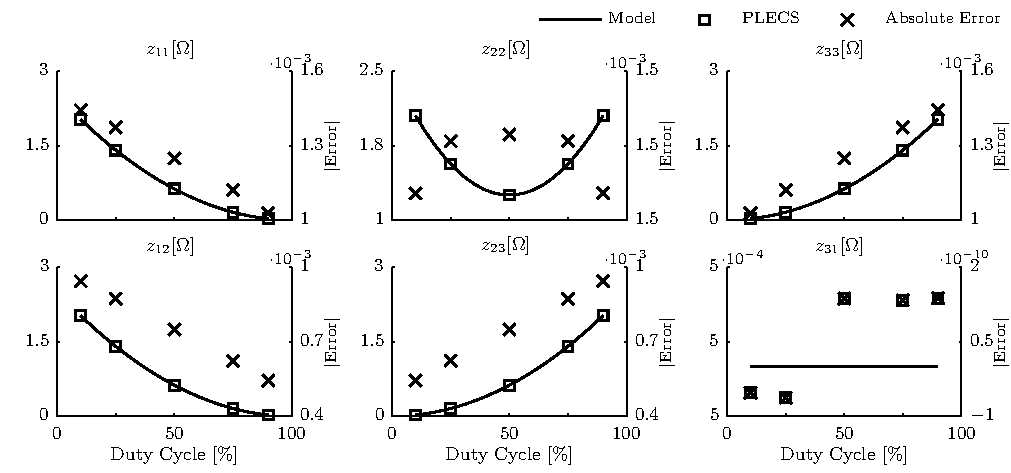
\includegraphics[page=1]{APEC_SIM_big}
  \centering
  \caption{SSL comparison between PLECS simulation and the proposed model.}
  \label{fig:sim_ssl}
\end{figure*}


\begin{figure*}[t]
  %\includegraphics[page=3]{APEC_SIM_big}
  \centering
  \caption{FSL comparison between PLECS simulation and the proposed model.}
  \label{fig:sim_fsl}
\end{figure*}

